
\documentclass[11pt,letterpaper]{article}

%\usepackage{cogsci}
%\usepackage{pslatex}
\usepackage{caption}
\usepackage{subcaption}
\usepackage{graphicx}
\usepackage{apacite}
\usepackage{color}
\usepackage{gb4e}
\usepackage{booktabs}
\usepackage{fullpage}


\definecolor{Red}{RGB}{255,0,0}
\newcommand{\red}[1]{\textcolor{Red}{#1}}
\newcommand{\jd}[1]{\textcolor{Red}{[jd: #1]}} 

\newcommand{\eref}[1]{(\ref{#1})}
\newcommand{\tableref}[1]{Table \ref{#1}}
\newcommand{\figref}[1]{Fig.~\ref{#1}}
\newcommand{\appref}[1]{Appendix \ref{#1}}
\newcommand{\sectionref}[1]{Section \ref{#1}}

\title{The natural distribution of \emph{or} -- scalar implicatures are few and far between}
 
%\author{{\large \bf Judith Degen (jdegen@stanford.edu)} \\
%  Department of Linguistics, 450 Serra Mall \\
%  Stanford, CA 95305 USA
%  \AND {\large \bf Neele Witte (XXX@XXX)} \\
%  XXX \\
%  XXX
%  \AND {\large \bf Michael Franke (XXX@XXX)} \\
%  XXX \\
%  XXX}

\author{Judith Degen, Neele Witte, Michael Franke}
\date\today

\begin{document}

\maketitle


\begin{abstract}


\textbf{Keywords:} 
\emph{or}; disjunction; scalar implicature; corpora; experimental pragmatics
\end{abstract}


\section{Introduction}

\jd{Why it's high time to look at \emph{or} in corpora of naturally occurring speech.}

\cite{degen2015}

\section{Corpus database}
\label{sec:database}

\jd{description fo corpus and motivation for using naturally occurring speech}

\subsection{Methods}

\jd{extraction patterns}

\subsection{Results}

\jd{overview of data; qualitative description of cases}


\section{Experiment 1: crowd-sourcing the location of \emph{but not both}}


\subsection{Methods}

\subsubsection{Participants}

\jd{XXX} participants were recruited via Amazon's Mechanical Turk and paid \jd{XXX} for their participation.

\subsubsection{Materials and Procedure}

Each of the 1244 sentences containing \emph{or} from the database described in \sectionref{sec:database} was shown to participants alongside \jd{XXX} lines of context. Arrows pointed to the space after every word in the sentence that occurred after \emph{or}, and participants were asked to indicate the best location for \emph{but not both} by clicking on one of the arrows.\footnote{The full experiment is available at \jd{XXX}.} If there was no good location, participants were nevertheless forced to provide a judgment, but there was a \emph{no good location} checkbox that they could click.

In order to familiarize them with the task, participants first completed two practice trials that they received feedback on before proceeding to the main experiment. See \figref{fig:exp1-task} for the two practice trials and an example of a target trial. The sentences were batched into \jd{XX} lists of 30 cases each and one additional list of 14 cases \jd{neele, stimmt das?}. Each participant completed 2 practice trials and 30 target trials.

\begin{figure}
\centering 
\begin{subfigure}{.7\textwidth}
\fbox{\includegraphics[width=\textwidth]{pics/exp1-example1.png}}
\caption{Practice trial 1.}
\end{subfigure}

\begin{subfigure}{\textwidth}
\fbox{\includegraphics[width=\textwidth]{pics/exp1-example2.png}}
\caption{Practice trial 2.}
\end{subfigure}

\begin{subfigure}{\textwidth}
\fbox{\includegraphics[width=\textwidth]{pics/exp1-trial.png}}
\caption{Example target trial.}
\end{subfigure}

\caption{Example practice and target trials in Exp.~1.}
\label{fig:exp1-task}

\end{figure}

\subsection{Data pre-processing and exclusion}

Each case received nine judgments, resulting in 11,196 data points. We excluded 378 trials on which participants inserted  \emph{but not both} immediately after \emph{or}, e.g.~\emph{do you work for a big or but not both a little place?}. This exclusion was motivated by these sentences resulting in guaranteed gibberish. After exclusion, 10,818 data points remained for analysis. \tableref{tab:casehist} shows the distribution of number of data points per case.  Only in one case did participants very consistently insert  \emph{but not both} right after \emph{or}. This case is shown in \eref{bador} \jd{neele, were there any other exclusion criteria?}

\begin{table}
\caption{Number of data points per case after removing cases where  \emph{but not both} was inserted immediately after \emph{or}.}
\begin{tabular}{l c c c c c}
\toprule
Number of data points per case &  1 &   6 &   7 &   8 &   9 \\
\midrule
Number of cases &  1 &  8 & 42 & 262 & 931 \\
\bottomrule
\end{tabular}
\label{tab:casehist}
\end{table}

\begin{exe}
	\ex\label{bador}  
\end{exe}

In order to select the final sentences to use in the scalar implicature experiment (Exp.~3), we computed the ``best response'' under four different selection criteria for each case:

\begin{enumerate}
	\item \textbf{Modal Response}: the most frequently given response
	\item \textbf{Most Frequent Good Location Response}: the response with greatest frequency of ``good location'' responses
	\item \textbf{Greatest Proportion Good Location Response}: the response with greatest proportion of ``good location'' responses \jd{wait how is this one different from the frequency one again?}
	\item \textbf{Closest to Or Response}: the response with the minimum distance between \emph{or} and \emph{but not both}
\end{enumerate}

\subsection{Results and discussion} 

We begin by analyzing the \emph{no good location} responses before proceeding to the selection of best responses.

\subsubsection{\emph{No good location} responses}

Overall, \jd{XX} of the \jd{XX} data points received a \emph{no good location} response. This number is quite high. If we take the lack of a natural location for \emph{but not both} as evidence that the \emph{and} sentence is not a viable alternative, this suggests that most sentences with \emph{or} do not compete with the corresponding stronger sentence with \emph{and}. This aligns with claims made by \jd{XX cite and maybe move to GD?}. A histogram of \emph{no good location} responses by item is shown in \figref{fig:nogoodlocation}.

\begin{figure}
	\includegraphics{pics/nogoodlocation-histogram.pdf}
\end{figure}

In order to provide an intuition for the data, and to probe our introspective judgments about the reasonableness of assigning a \emph{no good location} response, we list 3 cases each that received low ($<$ 10\%), medium (40-60\%) and high ($>$ 90\%) proportions of \emph{no good location} responses, respectively.
% CONTINUE HERE ONCE NEELE GIVES YOU THE RIGHT FILE TO WORK WITH

\begin{exe}
	\ex Low proportion
	\begin{xlist}
		\ex
		\ex
		\ex
	\end{xlist}	
	\ex Medium proportion
	\begin{xlist}
		\ex
		\ex
		\ex
	\end{xlist}	
	\ex High proportion
	\begin{xlist}
		\ex
		\ex
		\ex
	\end{xlist}			
\end{exe}

\subsubsection{Best response selection}

Of the 1244 cases, the best response was the same by all four selection criteria in 520 (42\%) of cases. An additional 107 (9\%)  of cases  had overlap in at least the Modal Response and the Closest to Or Response. A few examples are listed in \eref{completeoverlapexs}:

\begin{exe}
	\ex\label{completeoverlapexs}
	\begin{xlist}
		\ex Well, I guess I have used it once or twice \textbf{but not both}.
		\ex You know if it's informal I'd probably choose something, I mean, just like hamburgers or steaks \textbf{but not both} out on the grill because that's a lot of fun.
		\ex Even a bad school is a good school up here, where, if I lived in New York City or Washington DC \textbf{but not both}, uh, I would seriously consider moving if I had a child.
	\end{xlist}
\end{exe}

 

For cases that had overlap in both the Modal Response and the Closest to Or Response, that best response was selected (627 cases) to occur in the scalar implicature experiment (Exp.~3). In the remaining 617 cases, manual inspection of a random sample of 50 cases suggested that there is no general rule for selecting the best response. We therefore ran a second norming experiment on these remaining 617 cases in which we directly asked participants to compare two best responses and select the better one.



\jd{THE FOLLOWING REQUIRES CLEANUP. KEEP OR THROW OUT?}
To give the reader an intuition , we list 3 cases where the Modal Response and the Closest To Or Response differed in \tableref{nooverlapexs}.

\begin{table}
\caption{For each of 4 cases, number of total responses given alongside the modal response and the response that placed \emph{but not both} closest to \emph{or}.}
\centering
\begin{tabular}{l p{7cm} p{7cm}}
	\toprule
	\# of responses & Modal Response & Closest to Or Response \\
	\midrule
	4 & i wonder, i wonder how, how the civil system or the court system must differ between there and say where i am in minneapolis \textbf{but not both}  & i wonder, i wonder how, how the civil system or the court system \textbf{but not both} must differ between there and say where i am in minneapolis  \\
	4 & all we, all i do is, uh, keep a list of things like debts that are outstanding and every two or three months update that and every once in a while make a list of what we spent that month  \textbf{but not both} & all we, all i do is, uh, keep a list of things like debts that are outstanding and every two or three  \textbf{but not both} months update that and every once in a while make a list of what we spent that month\\
	3 & i, i mean i could have had that or a down payment on a new car \textbf{but not both} & i, i mean i could have had that or a down payment \textbf{but not both} on a new car\\
	\bottomrule
\end{tabular}
\end{table}

\begin{table}
\centering
\caption{Number of cases with overlap in best response by at least three criteria. The remaining 485 (39\%) of cases had overlap in fewer than three criteria.}
\begin{tabular}{l c c c c c}
\toprule
 & complete & MFP & MFC & MPC & FPC \\
\midrule
	Modal & $\surd$ & $\surd$ & $\surd$ & $\surd$ &  \\
	Freq &  $\surd$ & $\surd$ &  $\surd$ &  & $\surd$ \\	
	Prop & $\surd$ & $\surd$ & & $\surd$ & $\surd$ \\	
	Close & $\surd$ & & $\surd$ & $\surd$ & $\surd$ \\	
\midrule
Total & 520 & 133 & 78 & 16 & 12	\\
\bottomrule	
\end{tabular}
\end{table}

\section{Experiment 2: crowd-sourcing direct comparisons between \emph{but not both} locations}


\subsection{Methods}

\subsubsection{Participants}

\jd{XXX} participants were recruited via Amazon's Mechanical Turk and paid \jd{XXX} for their participation.


\subsubsection{Procedure}

The procedure was identical as in Exp.~1, with the exception of the task itself. Instead of inserting \emph{but not both}, participants were asked to compare two sentences and select the one that sounds better. Before the main experiment, participants completed two practice trials that they received feedback on. See \figref{fig:exp2-task} for the two practice trials and an example of a target trial. Each participant completed 30 trials.

\begin{figure}
\centering 
\begin{subfigure}{.7\textwidth}
\fbox{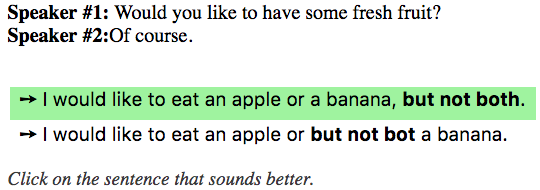
\includegraphics[width=\textwidth]{pics/exp2-example1.png}}
\caption{Practice trial 1.}
\end{subfigure}

\begin{subfigure}{\textwidth}
\fbox{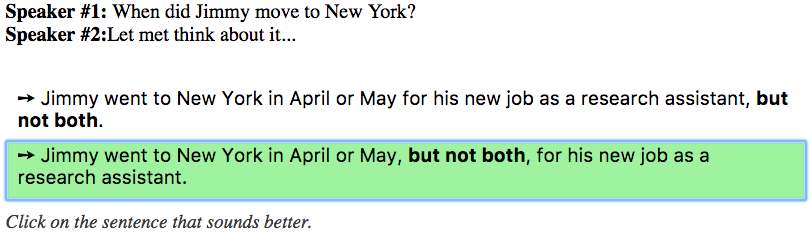
\includegraphics[width=\textwidth]{pics/exp2-example2.png}}
\caption{Practice trial 2.}
\end{subfigure}

\begin{subfigure}{\textwidth}
\fbox{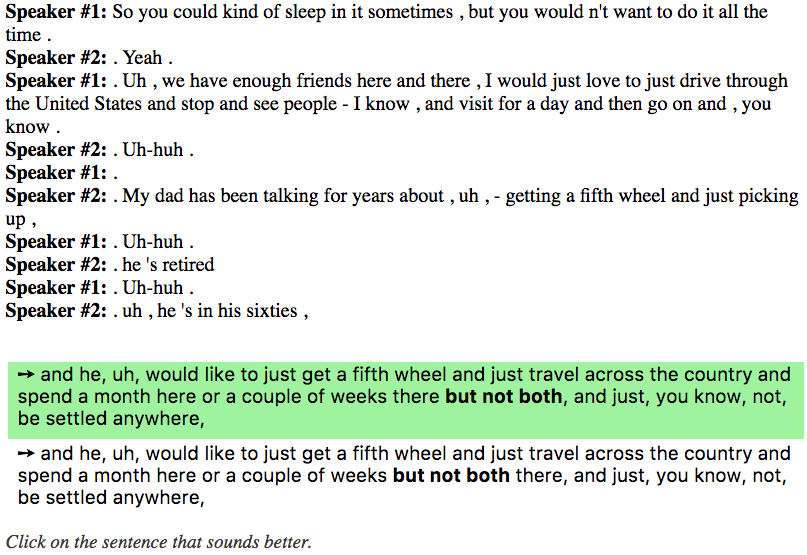
\includegraphics[width=\textwidth]{pics/exp2-trial.png}}
\caption{Example target trial.}
\end{subfigure}

\caption{Example practice and target trials in Exp.~2.}
\label{fig:exp2-task}

\end{figure}

\subsubsection{Materials}

Only the 617 cases that did not yield overlap in at least the Modal Response and the Closest to Or Response in Exp.~1 were included in this experiment. For each of these cases, we presented participants with the Modal Response and the Closest to Or Response to choose from if there was not more than one Modal Response (564 cases). If there was more than one Modal Response but only one Most Frequent Good Location Response, we presented participants with the comparison between Closest to Or and Most Frequent Good Location (29 cases). If there was more than one Modal Response but only one Most Frequent Good Location Response, we presented participants with the comparison between Closest to Or and Most Frequent Good Location (8 cases). For the remaining 16 cases, we hand-selected the best response.

\subsection{Results}

Each case received seven judgments. The resulting dataset is provided at \jd{XXX}. \tableref{tab:exp2results} shows the number and percentage of Comparison vs.~Closest to Or sentences that constituted the majority response for each case. Across all three groups, the comparison sentence was chosen more frequently than the Closest to Or sentence, but as our manual inspection of the random sample in Exp.~1 already suggested, there was no general rule for which sentence to choose. 

\begin{table}
\centering
\caption{Number and percentage of sentences selected in Exp.~2. when there was not more than one \textbf{Modal Response}, not more than one Most Frequent Good Location Response (\textbf{MFGLR}), and not more than one Greatest Proportion Good Location Response (\textbf{GPGLR}).}
\begin{tabular}{l r r r r r r}
\toprule
& \multicolumn{6}{c}{Comparison sentence}\\
 & \multicolumn{2}{c}{Modal Response} & \multicolumn{2}{c}{MFGLR} & \multicolumn{2}{c}{GPGLR}\\
\midrule
Selected Comparison & 418 & 74\% & 18 & 62\% & 5 & 63\%\\
Selected Closest to Or & 146 & 26\% & 11 & 37\% & 3 & 38\%\\
\bottomrule
\end{tabular}
\label{tab:exp2results}
\end{table}






%
%
%\begin{table}[!ht]
%\begin{center} 
%\caption{Sample table title.} 
%\label{sample-table}  
%\vskip 0.12in
%\begin{tabular}{ll} 
%\hline
%Error type    &  Example \\
%\hline
%Take smaller        &   63 - 44 = 21 \\
%Always borrow~~~~   &   96 - 42 = 34 \\
%0 - N = N           &   70 - 47 = 37 \\
%0 - N = 0           &   70 - 47 = 30 \\
%\hline
%\end{tabular} 
%\end{center} 
%\end{table}
%

%\begin{figure}[ht]
%\begin{center}
%\fbox{CoGNiTiVe ScIeNcE}
%\end{center}
%\caption{This is a figure.} 
%\label{sample-figure}
%\end{figure}


\section{Experiment 3: crowd-sourcing scalar implicatures}


\subsection{Methods}

\subsubsection{Participants}

\jd{XXX}

\subsubsection{Materials}

\jd{XXX}

\subsubsection{Procedure}

\jd{XXX}

\subsection{Results}

\jd{XXX}

\section{General discussion}

\appendix

\section{Hand-selected \emph{but not both} sentences}
\label{app:handselectedbnb}

For the 16 sentences from Exp.~1 that did not receive a clear best location assignment for \emph{but not both}, the lead author hand-selected the best location, resulting in the following 16 sentences.

\begin{exe}
	\ex List of 16 manually annotated \emph{but not both} sentences
	\begin{xlist}
	\ex and i think that the people who are strongly in favor of the death penalty are really working from that gut level. uh, you know, whether it be a biblical force, uh, you know, the eye for an eye, a tooth for a tooth, a life for a knife, life type logic or just, uh, uh, some sort of anger at putting peop-, putting, uh, murderers up in federal pens for the rest of their life, \textbf{but not both}, uh, while we foot the bill.
	\ex we've set a budget for each, you know, household expenses, or food, \textbf{but not both}, and clothing and entertainment and then our, our own fun money and just stuff like that
	\ex so i guess i've done probably, uh, i'd say seven or eight \textbf{but not both} of them.
	\ex like, would you go over and spend a lot of time in one place, or travel to whole bunch of different places \textbf{but not both} in one week.
	\ex uh, i think that the judges should be leftd to do most of the sentencing, simply because, uh, there is always, uh, there is, there is always a jury that might be swayedb, uh, by the moment, uh, to either to be too lenient or too vengeful, \textbf{but not both}, i guesse.
	\ex we use it more for just writing programs when we need to or, um, doing research, \textbf{but not both}, looking at the speech signal and then doing writing, and also as a just as a terminal,
	\ex and there are parts of downtown or near downtown dallas \textbf{but not both} that are under water right now, i guess,
	\ex the question was, um, what, what is your opinion of youth, uh, spending a year or two \textbf{but not both} in, in public service.
	\ex but if we're going to have a meeting, where we're having the attorneys come in, or people from, uh, other party's attorneys and stuff \textbf{but not both}, then i normally dress up.
	\ex well i remember last year, or the year before, \textbf{but not both}, uh, we had ice and snow, uh, uh,
	\ex see, it have been like nineteen sixty-seven or sixty-eight, \textbf{but not both}, um,
	\ex because there was an article or a story \textbf{but not both} done awhile ago that, uh, trash, uh, the telephone books are the type of thing that don't break down over a long period of time.
	\ex she's had about four or five litters \textbf{but not both}.
	\ex and, and drink wise they have kool-aid, milk or water but bot both. normally.
	\ex but, uh, in the long run, it seems to me, it's kind of like what they keep talking about the, uh, the aids testing with doctors or dentists \textbf{but not both} and things and how that, you know,
	\ex uh, i don't remember what they call it, sort of like a positive, negatives or some, some kind of word they use when a, uh, you get a, uh, a positive indication of drugs, but there's not really, there weren't really any there \textbf{but not both}.
	\end{xlist}
\end{exe}

\bibliographystyle{apacite}

\setlength{\bibleftmargin}{.125in}
\setlength{\bibindent}{-\bibleftmargin}

\bibliography{bibs}


\end{document}
